\section{Wechselstromrechnung}
	\subsection{Allgemein zeitabhängige Grössen}
	\begin{tabular}{|ll|ll|}
    \hline
	\multicolumn{2}{|l}{Arithmetischer Mittelwert, Gleichwert, Linearer MW} 
	    	& \multicolumn{2}{l|}{$X_0 = \overline{X} = X_m = \frac {1} {T} \int\limits_{t_0}^{t_0+T}
	    	x(t)dt$} \\
	\hline
	Leistung, Mittelwert des Quadrats
		& $X^2 = \frac {1} {T} \int\limits_{t_0}^{t_0+T} x^2(t)dt$ 
		& MW $n$. Ordnung
		& $X^n = \frac {1} {T} \int\limits_{t_0}^{t_0+T} x^n(t)dt$ \\
	\hline
	Mittlere Leistung
			& \multicolumn{3}{l|}{$P= \frac{1}{T}\int\limits_{t_0}^{t_0+T} p(t) \diff t = \frac{1}{T}\int\limits_{t_0}^{t_0+T} u(t) \cdot i(t) \diff t = 
			R\cdot \frac{1}{T}\int\limits_{t_0}^{t_0+T} i^2(t) \diff t =
			\frac{1}{R} \cdot \frac{1}{T}\int\limits_{t_0}^{t_0+T} u^2(t) \diff t
			$}\\
		\hline
	Effektivwert, RMS 
		& $X = \sqrt{X^2} = \sqrt{\frac{1}{T} \int\limits ^{t_0+T}_{t_0}{x^2(t)dt}}$
		& Gleichrichtwert 
		& $X_{|m|} = \bar{|X|} = \frac{1}{T} \int\limits_{t_0}^{t_0+T}{|x(t)| dt}$ \\
	\hline
   	\end{tabular}
   	
   	\subsection{Grundelemente}
   		\begin{tabular}{p{1.5cm} p{4.3cm} |p{1.5cm} p{4.3cm}| p{1.5cm} p{4.3cm}}
   	   		\multicolumn{2}{l}{\textbf{Ohmscher Widerstand R}}
   	   			& \multicolumn{2}{l}{\textbf{Kapazitität C}}
   	   			& \multicolumn{2}{l}{\textbf{Induktivität L}} \\
   	   		\multicolumn{2}{l}{$u$ und $i$ können sprunghaft ändern}
   	   			& \multicolumn{2}{l}{$\mathbf{u}$ \textbf{kann nicht sprunghaft ändern}}
   	   			& \multicolumn{2}{l}{$\mathbf{i}$ \textbf{kann nicht sprunghaft ändern}} \\
   	   	
   	   		\multirow{2}{1.5cm}{
   				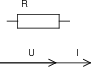
\includegraphics[width=1.5cm]{./images/zeigerdiag-r.png}}
   				& $u(t) = R \cdot i(t)$ 
   				& \multirow{2}{1.5cm}{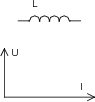
\includegraphics[width=1.5cm]{./images/zeigerdiag-l.png}}
   				& $u(t) = \frac{1}{C} \int\limits_0^t i(\tau) d\tau + u(0)$
   				& 
   				\multirow{2}{1.5cm}{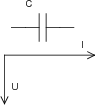
\includegraphics[width=1.5cm]{./images/zeigerdiag-c.png}}
   				&$u(t) = L \frac{di(t)}{dt}$\\
   				
   				&$i(t) = \frac{u(t)}{R}$
   				& & $i(t) = C \frac{d u(t)}{dt}$
   				& & $i(t) = \frac{1}{L} \int\limits_0^t u(\tau) d\tau + i(0)$\\
   				
   				& $\underline{Z}_R = R$
   				& & $\underline{Z}_C = \frac{1}{j \omega C} = - \frac{j}{\omega C}$
   				& & $\underline{Z_L} = j \omega L$\\
   				
   				\parbox{1.7cm}{\small{nicht linear:}}
   				& $R_=(u) = \frac{U}{I(u)}, r_D = \frac{\diff U}{\diff I}\lvert_{U_0}$
   				& & $X_C = -\frac{1}{\omega C} \quad B_C = \omega C$
   	   			& & $X_L = \omega L
   	   			\quad B_L = -\frac{1}{\omega L}$ \\
   	   			
   	   			& $P=I^2 \cdot R = \frac{U^2}{R}$
   	   			& & $Q_C= - U^2 \cdot \omega C = - \frac{I^2}{\omega C}$
   	   			& & $Q_L= I^2 \cdot \omega L = \frac{U^2}{\omega L}$\\
   	   			
   	   			& & & $W_C=\frac12 C U_C^2$
   	   			& &$W_L=\frac12 L I_L^2$
   	   	\end{tabular}
   	
   		\subsection{Vorgehen bei Schaltvorgängen}
   		\fbox{$u(t) =U_E + (U_A - U_E) e^{\frac{-t}{\tau}} \qquad i(t) =I_E + (I_A - I_E) e^{\frac{-t}{\tau}} \qquad
   		\tau = C R = \frac{L}{R}
   		\qquad \underbrace{X_A}_{Anfang} = \lim\limits_{t
   		 \rightarrow 0^+} x(t) \qquad \underbrace{X_E}_{Ende} =
   		 \lim\limits_{t \rightarrow \infty} x(t)$} $\qquad$\\
   		 \textbf{Beachte:} Spannung an $C$ und Strom an $L$ können nicht sprunghaft ändern. \\
   		 Zur Bestimmung von R alle Quellen ausschalten und Belastung von Speicherelement her betrachten 

	\subsection{Komplexe Darstellung sinusförmiger Vorgänge}
		Momentanwert in $\mathbb{R}$: \fbox{$a(t) = \hat{A} \cos(\omega t + \varphi)$} \quad
		Momentanwert in $\mathbb{C}$: \fbox{$\underline{a}(t) = \hat{A} e^{j \varphi} e^{j
		\omega t} = \underline{\hat{A}}e^{j
				\omega t}$} $\quad$ 
		Amplitude in $\mathbb{C}$: \fbox{$\underline{\hat{A}} = \hat{A} e^{j \varphi}$}\\
		
		Differentiation: $\frac{d}{dt} \underline{a}(t) = \underbrace{j \omega \underline{\hat{A}}}_{\underline{\hat{A}}_d}\cdot \e^{\im \omega t}$ $\qquad$ 
		Integration: $\int \underline{a}(t) dt = \underbrace{\frac{\underline{\hat{A}}}{j \omega}}_{\underline{\hat{A}}_i}\cdot \e^{\im \omega t}$

	\subsection{Begriffe der Impedanz und Admitanz}
		\begin{tabular}{lllll}
		Scheinwiderstand & & $Z = \frac{U_{eff}}{I_{eff}} $ & $ =
		\sqrt{R^2+X^2}$ & Ohm\\ Komplexer Widerstand & Impedanz & $\underline Z = R + jX = Z \cdot e^{j \varphi}$ 
		& $  = \dfrac{\underline{U}}{\underline{I}} = \dfrac{\underline{U}^2}{\underline{S}^*} = 
		\dfrac{\underline{S}}{\underline{I}^2}$ & Ohm\\
		Komplexer Leitwert & Admittanz & $\underline Y = G + jB =
		\frac{1}{\underline Z} = \frac{1}{Z}e^{-j\varphi}$ & $= \frac{\underline{I}}{\underline{U}}$ &  Siemens\\
		Wirkwiderstand & Resistanz & $R = \Real(\underline Z) $ & $ = Z
		\cdot cos(\varphi)$ & Ohm\\
		Wirkleitwert & Konduktanz & $G = \Real(\underline Y) $ & $ \neq \frac{1}{R}$ &
		Siemens\\
		Blindwiderstand & Reaktanz & $X = \Imag(\underline Z) $ & $ = Z
		\cdot sin(\varphi)$ & Ohm\\
		Blindleitwert & Suszeptanz & $B = \Imag( \underline Y) $ & $ \neq \frac{1}{X}$
		& Siemens\\
		Phasenverschiebung & & $\varphi = \varphi_u - \varphi_i =
		\arctan\left(\frac{\Imag(\underline{Z})}{\Real(\underline{Z})}\right)$ & &
		Radiant\\
		
		\end{tabular}
	
	\subsubsection{Parallel \& Reihen-Ersatzschaltung (mit Vorsicht geniessen)}
		
	\begin{centering}
			
	\begin{tabular}{|l|c|c|}
		\hline
			& Parallel-Ersatzschaltung & Reihen-Ersatzschaltung \\
		\hline
			Schaltbild & 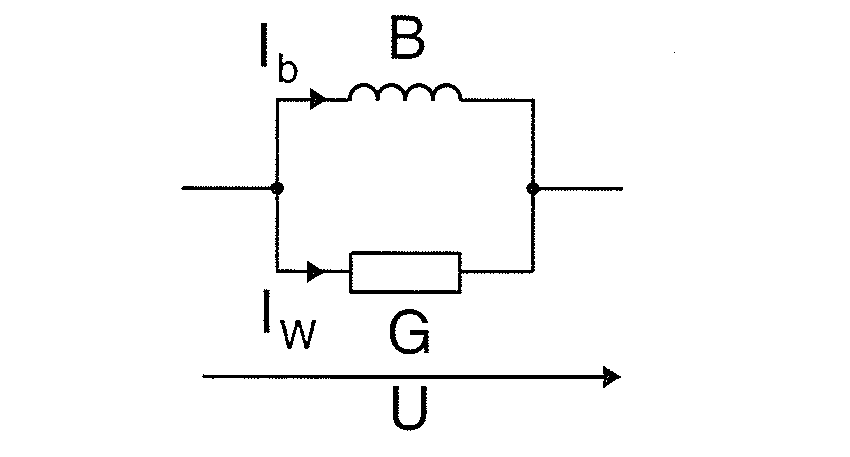
\includegraphics[width=3cm]{./images/RL_parallel.png} &
			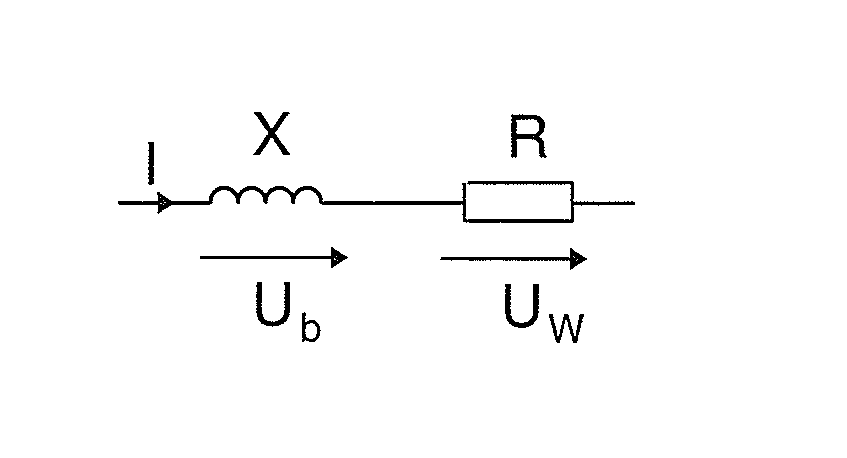
\includegraphics[width=3cm]{./images/RL_Seriel.png}\\
		\hline
			komplexer Widerstand & & $\underline{Z}=R+jX$\\
			komplexer Leitwert & $\underline{Y}=G+jB$ &\\
		\hline
			Scheinwiderstand & & $Z=\sqrt{R^2+X^2}$\\
			Scheinleitwert & $Y=\sqrt{G^2+B^2}$ & \\
		\hline
			Wirkwiderstand & & $R=Z\cos\varphi=\frac{U_W}{I}$\\
			Wirkleitwert & $G=Y\cos\varphi_{_Y}=\frac{I_W}{U}$&\\
		\hline
			Blindwiderstand & & $X=Z\sin\varphi=\frac{U_b}{I}$\\
			Blindleitwert & $B = Y\sin\varphi_{_Y} = \frac{I_b}{U}$&\\
		\hline
			komplexe Leistung & $\underline{S}=
			\underline{Y^*}U^2=\left(G-jB\right)U^2$& $\underline{S}=\underline{Z}I^2=\left(R+jX\right)I^2 = \frac{U^2}{\underline{Z}^{\ast}}$\\
			Wirkleistung & $P=I_W U=\frac{I{_W}{^2}}{G}=U^2G$ &
			$P=U_WI=\frac{U{_W}{^2}}{R}=I^2R$ \\
			Bildleistung & $Q=-I_bU=\frac{-I{_b}{2}}{B}=-U^2B$ & $Q = U_bI =
			\frac{U{_b}{^2}}{X}=I^2X$\\
			Scheinleistung & $S=UI=U\sqrt{I{_W}{^2}+I{_b}{^2}}$ & $S=UI =
			I\sqrt{U{_W}{^2}+U{_b}{^2}}$\\
		\hline
			Wirkfraktor & $\cos\varphi_{_Y}= \frac{G}{Y}$ & $\cos\varphi=\frac{R}{Z}$\\
			Blindfaktor & $\sin\varphi_{_Y}= \frac{B}{Y}$ & $\sin\varphi=\frac{X}{Z}$\\
		\hline
			Wirkstrom & $I_W=I\cos\varphi_{_Y}=GU$ & \\
			Wirkspannung & & $U_W = U\cos\varphi =R \cdot I$ \\
		\hline
			Blindstrom & $I_b = -I \sin\varphi_{_Y} = BU$ & \\
			Blindspannung & & $U_b=U\sin\varphi=X\cdot I$\\
		\hline
	\end{tabular}\\
	\end{centering}

\subsection{Leistungen und Energie}
	\begin{tabular}{ll}
   		\parbox{4cm}{
   			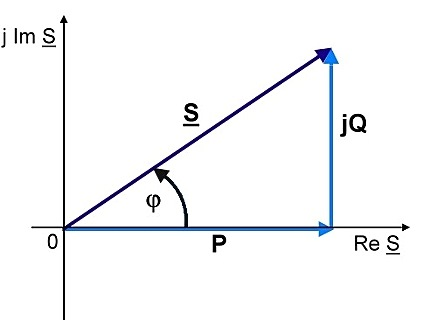
\includegraphics[width=4cm]{./images/zeigerdiag-leistungen.png}}
   		& \parbox{14cm}{
			\begin{tabular}{p{3cm}p{4.5cm}p{5.5cm}}
	      		\multirow{2}{4cm}{Komplexe Leistung}  &
	      			$ \underline{S} = P + jQ$  &\\
	      			& \multicolumn{2}{l}{$ \underline{S} = \underline{U} \cdot \underline{I}^\ast = U\cdot I \cdot e^{j(\varphi_u-\varphi_i)} = \frac{\underline{U}^2}{\underline{Z}^*} = \underline{I}^2 \cdot \underline{Z} = \underline{U}^2\cdot\underline{Y}^*$}\\
				Scheinleistung
					& $ S = | \underline{S} | = U I = \frac{U^2}{Z} = I^2 Z$ 
					& \\
				Wirkleistung
					& $ P = \Real(\underline{S}) = U I \cos(\varphi) $ \\
				Blindleistung 
					& $ Q = \Imag(\underline{S}) = U I \sin(\varphi) $
					& Kapazitiv: $Q < 0$; induktiv: $Q > 0$ \\
				Leistungsfaktor
					& $\cos \varphi = \frac{P}{S} = \frac{P}{UI}$ \\
			\end{tabular}}
   	\end{tabular}
\subsubsection{Leistungsanpassung von komplexen Quellen}
	\begin{equation*}
		\boxed{\underline{Z}_L = \underline{Z}_i^{\ast}} \qquad \underline{Y}_L = \underline{Y}_i^{\ast} \qquad P_{max} = \frac{U_q^2}{4R_i} = \frac{I_q^2 R_i}{4} 
	\end{equation*}   	

\subsubsection{Blindleistungskompensation}
\begin{tabular}{p{4cm}p{4cm}p{4cm}p{6cm}}
\begin{minipage}{4cm}
    	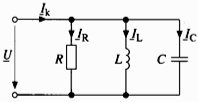
\includegraphics[width=3.5cm]{./images/Parallelkompensation.png}
    	\end{minipage}
	& \begin{minipage}{4cm}
    	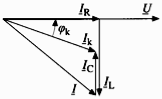
\includegraphics[width=3.5cm]{./images/Blindstromkompensation.png}
    	\end{minipage}
	& \begin{minipage}{4cm}
    	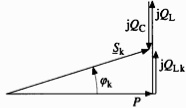
\includegraphics[width=3.5cm]{./images/Blindleistungskompensation.png}
    	\end{minipage} 
	& \begin{minipage}{6cm} 
		$$Q_{L} = P \cdot \tan{\varphi}$$     
		$$Q_{Lk} = P \cdot \tan{\varphi_k}$$
		$$Q_C = Q_{Lk} - Q_L$$
		$$C = -\frac{Q_C}{\omega U^2}$$
		\end{minipage}
\end{tabular}

\subsection{Systematische Netzwerkanalyse}

\subsubsection{Netzwerkgleichungen, Integro-Differentialgleichungen}
Die Netzwerkgleichungen werden nach den selben Regeln aufgestellt, wie für Widerstandsnetze, wobei die Energiespeicher (C,L,M) im Zeitbereich aufgeschrieben werden mit $\int f(t) dt$ und $\frac{d}{dt} f(t)$ Siehe 2.2 Grundelemente.	\\ 

%\subsubsection{Zweigstrommethode / Kreisstrommethode / Maschenstrommethode}
\begin{tabular}{p{9cm}|p{9cm}}
	\begin{minipage}{9cm}
		%\textbf{Zweigstrommethode}\\
		\subsubsection{Zweigstrommethode}		
		\begin{list}{$\bullet$}{\setlength{\itemsep}{0cm} \setlength{\parsep}{0cm} \setlength{\topsep}{0cm}} 
		\item Maschengleichungen enthalten \textbf{Zweigströme} \\
		$\quad\Rightarrow$ Maschen- \& Stromknotengleichungen benötigt\\
		\item kann nicht in Matrizenform dargestellt werden\\  
        \end{list} 
		\hrule
		\vspace{0.2cm}
		%\textbf{Kreis- oder Maschenstrommethode} (s. Bilder rechts)\\
		\subsubsection{Kreis- oder Maschenstrommethode} (s. Bilder rechts)\\
		\begin{list}{$\bullet$}{\setlength{\itemsep}{0cm} \setlength{\parsep}{0cm} \setlength{\topsep}{0cm}} 
			\item Stromquellen in Spannungsquellen umwandeln.\\ $\underline{U}_q = \underline{I}_q \cdot \underline{Z}$\\[0.2cm]
			\textbf{Maschenstrommethode:}
			\item Maschengleichungen enthalten \textbf{Maschenströme}\\
			$\quad\Rightarrow$ nur Maschengleichungen benötigt\\[0.2cm]
			\textbf{Kreisstrommethode:}
		    \item \textcolor{brown}{Baum} verbindet alle \textcolor{red}{Knoten}, ist nie geschlossen
		    \item Aufzustellende \textcolor{green}{Kreise} bestehen immer aus beliebig
		    vielen \textcolor{brown}{Ästen} (Zweige vom Baum) und \textbf{einer Sehne} (Zweige die nicht zum Baum gehören)
		    \\
		    
	    \end{list}	
    \end{minipage} &
	\begin{minipage}{9cm}
    		\underline{Bild 1}\\
    		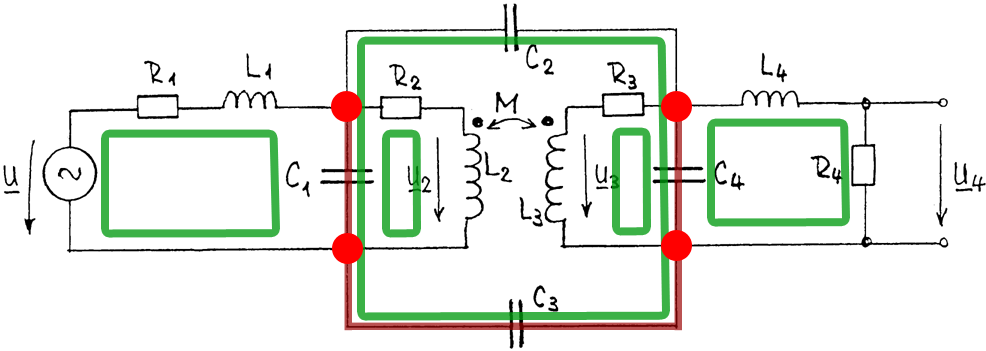
\includegraphics[height=3cm]{./images/netzwerkanalyse-kreisstrom2.png}\\
			\underline{Bild 2}\\
			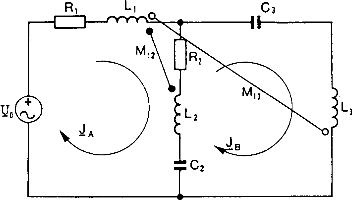
\includegraphics[height=3.5cm]{./images/netzwerkanalyse-maschenstrom.png}\\
    		\\
    		\\
    		\hrule
    \end{minipage}\\
\end{tabular} \\
\\ \\
\textbf{Matrix der Maschenstrommethode (Bild 2)}
$$\left[ \begin{array}{cc}
        R_1+R_2 +j \omega L_1 + \frac{1}{j \omega C_2} + j \omega L_2 - j 2
        \omega M_{12} 
    & -(R_2 + j \omega L_2 + \frac{1}{j \omega C_2} - j \omega M_{12} -
        j \omega M_{13}) \\
    -(R_2 + j \omega L_2 + \frac{1}{j \omega C_2} - j \omega M_{12} - j
        \omega M_{13})
    & R_2 + j \omega L_2 + j \omega L_3 + \frac{1}{j \omega C_2} +
        \frac{1}{j \omega C_3}
\end{array}\right] \cdot
\left[ \begin{array}{cc}
     \underline{J}_A \\ \underline{J}_B
     \end{array}\right] =
\left[ \begin{array}{cc}
     U_0 \\ 0
     \end{array}\right]$$
$$\textbf{Allgemein: }\left[ \begin{array}{cc}
       \text{Impedanzen $\underline{Z}$} \\
       \text{symmetrisch zur Diagonalen}
%       \text{Diagonale positiv, sonst negativ}
       \end{array}\right] \cdot \left[ \begin{array}{cc}
     \text{Maschenströme $\underline{J}$}
     \end{array}\right] =
\left[ \begin{array}{cc}
     \text{Spannungsquellen $\underline{U}$} \\
    \text{Gegenrichtung positiv, sonst negativ}
     \end{array}\right]$$

\subsubsection{Gegeninduktivitäten}
	\textbf{Kreis/Maschenstrom-Methode:}
	\begin{list}{$\bullet$}{\setlength{\itemsep}{0cm} \setlength{\parsep}{0cm} \setlength{\topsep}{0cm}} 
	
		\item {\textbf{Gekoppelte Induktivitäten innerhalb eines Kreises}:\\
		Da der ``eigene`` Kreisstrom $\underline{J}_K$ von jeder Spule auf die andere wirkt, erhält man Ausdrücke der Form $\pm 2 \im\omega M \cdot \underline{J}_K$ . Das positive Vorzeichen gilt, wenn die Spulen gleichsinnig im Kreis liegen.\\}
		\item {\textbf{Spannungsanteile aufgrund ``fremder`` Kreisströme:}\\
		Fliesst der ``fremde`` (induzierende) Strom bei der \textbf{Markierung hinein}, so hat er dieselbe
		Wirkung als wenn er bei der gekoppelten Spule in die \textbf{Markierung
		hineinfliessen würde}!}\\
		
	\end{list}

 	\textbf{Knotenpotential-Methode:}\\
	Die Netzwerkgleichungen können nicht ohne weiteres formu- liert werden, da hierzu die Zweigströme als Funktion der Knotenpotentiale vorliegen sollten. Man kann hierzu die Trafogleichungen entsprechend umformen oder eine Ersatzschaltung mit gesteuerten Quellen einführen.\\ \\
	\begin{minipage}{9cm}
		\textbf{Einfacher Spezialfall:}\\
			Sind bei einem Übertrager die einen Wicklungsenden miteinander verbunden - oder dürfen sie ohne Beeinflussung der restlichen Schaltung miteinander verbunden werden - so kann die Ersatzschaltung rechts verwendet werden.
	\end{minipage}
	\begin{minipage}{9cm}
	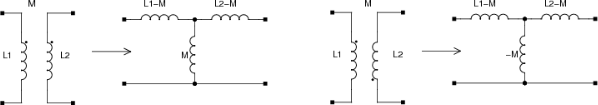
\includegraphics[width=9cm]{./images/netzwerkanalyse-kopplung-spulen.png}
	\end{minipage}




\subsubsection{Knotenpotentialmethode oder Trennbündelmethode}
\begin{tabular}{ll}
\parbox{6cm}{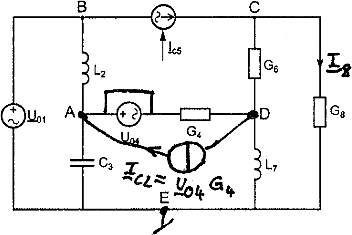
\includegraphics[width=6cm]{./images/netzwerkanalyse-knotenpotential.png}
	}
	& \parbox{12cm}{
	Gegeben: $\underline{I}_{C5} = k \underline{I}_8$
	\begin{itemize}
      \item Knoten B hat keine Gleichung, da $E_B = \underline{U}_{01}$
      \item Rechnung nur mit \textit{Admittanzen} (Leitwerten) $\underline{Y}
      = \frac{1}{\underline{Z}} = G + jB$
      \item Schema mit (idealen) \textit{Stromquellen}\\
      $\Rightarrow$ Spannungsquellen
      umwandeln $\underline{I}_q = \underline{U}_q \cdot \underline{Y}$
    \end{itemize}
$$\begin{bmatrix}
    G_4 + \frac{1}{j \omega L_2} + j \omega C_3 & 0 & -G_4 \\
    0 & G_6 + G_8 - \underbrace{k G_8}_{\underline{I}_{C5}} & -G_6 \\
    -G_4 & -G_6 & \frac{1}{j \omega L_7} + G_4 + G_6   
	\end{bmatrix} \cdot
\begin{bmatrix}
    \underline{E}_A \\ \underline{E}_C \\ \underline{E}_D
    \end{bmatrix} =
\begin{bmatrix}
    \underline{U}_{04} G_4 + \frac{\underline{U}_{01} }{j \omega L_2}\\ 
    0 \\
    -\underline{U}_{04} G_4 \end{bmatrix}$$    
	}
\end{tabular}

$$\textbf{Allgemein: }\left[ \begin{array}{cc}
       \text{Admittanzen $\underline{Y}$} \\
       \text{symmetrisch zur Diagonalen}
%       \text{Diagonale positiv, sonst negativ}
       \end{array}\right] \cdot \left[ \begin{array}{cc}
     \text{Knotenpotentiale $\underline{E}$}
     \end{array}\right] =
\left[ \begin{array}{cc}
     \text{Stromquellen $\underline{J}$} \\
    \text{Hineinfliessen positiv, sonst negativ}
     \end{array}\right]$$

\renewcommand{\arraystretch}{1.2}
\subsubsection{Aspekte zur Wahl der Methode}
\begin{tabular}{llllll}
	\multicolumn{3}{l}{\textit{Art der gegebenen Quellen}} & \multicolumn{3}{l}{\textit{Spezialitäten}}\\
	& Kreisstrom: & Spannungsquellen
	& Kreisstrom: & Gegeninduktivitäten \\
	& Knotenpotential: & Stromquellen 
	& Knotenpotential: & Gesteuerte Stromquellen \\
	
	\multicolumn{3}{l}{\textit{Anzahl Gleichungen}}
	& \multicolumn{3}{l}{\textit{Gesuchte Grössen}}\\ 
	& Kreisstrom: & $z-k+1-$ Anzahl idealer Stromquellen
	& Kreisstrom: &(Sehnen-) Ströme\\
	& Knotenpotential: &$k-1-$ Anzahl idealer Spannungsquellen
	& Knotenpotential: &(Knoten-) Spannungen

\end{tabular}

\renewcommand{\arraystretch}{\arraystretchOriginal}

	\input{idiotenseite/elektrotechnik/subsections/quellenverschiebung}

\subsection{Stern-Dreieck-Umwandlung}% \formelbuch{18}}
	%\begin{figure}
	  \begin{minipage}[lt]{7.5 cm}
	    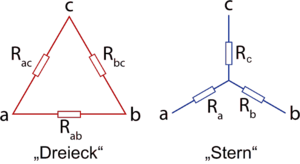
\includegraphics[width=6cm]{./images/stern-dreieck.png} 
	  \end{minipage}
	  \begin{minipage}[rt]{9.35 cm} %BASTEL!!
	  \begin{tabular}{ll}
	Umwandlung $\triangle \rightarrow Y$: 
		&$Z_{c} = \dfrac{Z_{ac} Z_{bc}}{Z_{ab}+Z_{bc}+Z_{ac}}$\\
	Umwandlung $Y \rightarrow \triangle$: 
		&$Y_{ac}=\dfrac{Y_{a} Y_{c}}{Y_{a}+Y_{b}+Y_{c}}$\\
	Bei gleichen Widerständen:
	&$R_Y = \frac{R_\triangle}{3}$ \\
	Bei gleichen Kapazitäten:
	&$C_Y = C_\triangle \cdot 3 $ \\
	Bei gleichen Induktivitäten:
	&$L_Y = \frac{L_\triangle}{3}$
	  \end{tabular}
	  \end{minipage}
	  
\newpage

\subsection{Impedanz-Transformationen}
Werden gebraucht, wenn Grundelemente variablen Werten unterliegen können. Bspw. wird $\omega$ variiert\\
%Immer zuerst die einfachere Variante (Serieschaltung: \underline{Z},
%Parallelschaultung: \underline{Y}) darstellen und daraus die andere Ortskurve herleiten. \\
Bei der Umwandlung von \underline{Z} nach \underline{Y} und umgekehrt handelt es sich um die
\textbf{komplexe Kehrwertfunktion}: 
\begin{itemize}
  \item $\underline{Y} = \frac{1}{\underline{Z}} \;
  ( \varphi_{_Z} = -\varphi_{_Y},  
  |\underline{Y}| = \frac{1}{| \underline{Z} |}) \qquad$
  (Unendlich ferner Punkt wird in den Ursprung abgebildet und umgekehrt)
  \item Verläuft die OK von \underline{Z} oberhalb der Re-Achse, so verläuft die OK von
  \underline{Y} unterhalb der Re-Achse und umgekehrt.
\end{itemize} 
\textbf{Konstruktion} der kreisförmigen Ortskurve (OK):
\begin{enumerate}

  \item Andere Orstkurve (komplexer Kehrwert) als Gerade darstellen. (Dient als Orientierungshilfe und zur Überprüfung)
  \textbf{Tipp}: $Z$ \& $Y$ in gemeinsames 		
  	Achsenkreuz eintragen. Skalierung entweder für $Z$ \& $Y$ unterschiedlich, oder normieren: $\underline{z} = \underline{Z} / R_0 \quad \underline{y} = \underline{Y} \cdot R_0$
  
  \item Extremalwerte berechnen und als Punkte $P_1, P_2$ darstellen. \\
	($P_1 = \underline{Z}_0 = \lim\limits_{x \rightarrow 0}\underline{Z}, \quad
	  P_2 = \underline{Z}_\infty = \lim\limits_{x \rightarrow \infty}\underline{Z} $ mit $x$ als veränderliche Grösse, z.B $x = \omega, R,L,C$)\\
	 Für das bestimmen der Winkel kann hier die andere Ebene zur Hilfe genommen werden. Achtung: $\varphi_{_Z} = -\varphi_{_Y}$
	 
  \item Mittelsenkrechte von $P_1, P_2$ konstruieren, deren Schnittpunkt mit Re- \textbf{oder}
  Im-Achse den Kreismittelpunkt $M$ ergibt. \\
  Mittels Betrachtung des Anfangswinkels ($\varphi_{Z_0} = - \varphi_{Y_0}$  oder
  $\varphi_{Z_\infty} = - \varphi_{Y_\infty}$) kann die Anfangsrichtung des Kreises in
  der Nähe des Ursprungs bestimmt werden und der ''falsche'' Mittelpunkt ($M_{Re}$ oder $M_{Im}$)
  ausgeschlossen werden.
  \item Ortskurve (Kreis mit Mittelpunkt $M$, schneidet $P_2$ und $P_1$) konstruieren
  \item In der $Z$-Ebende bewirkt ein weiteres serielles Element, dass die Ortskurve um deren komplexen Wert verschoben wird.\\
  Das gleiche gilt auch für weitere parallele Elemente in der $Y$-Ebene. (Bsp. siehe Grafik unten mit zusätzlichem $\underline{Z}$)
\end{enumerate}

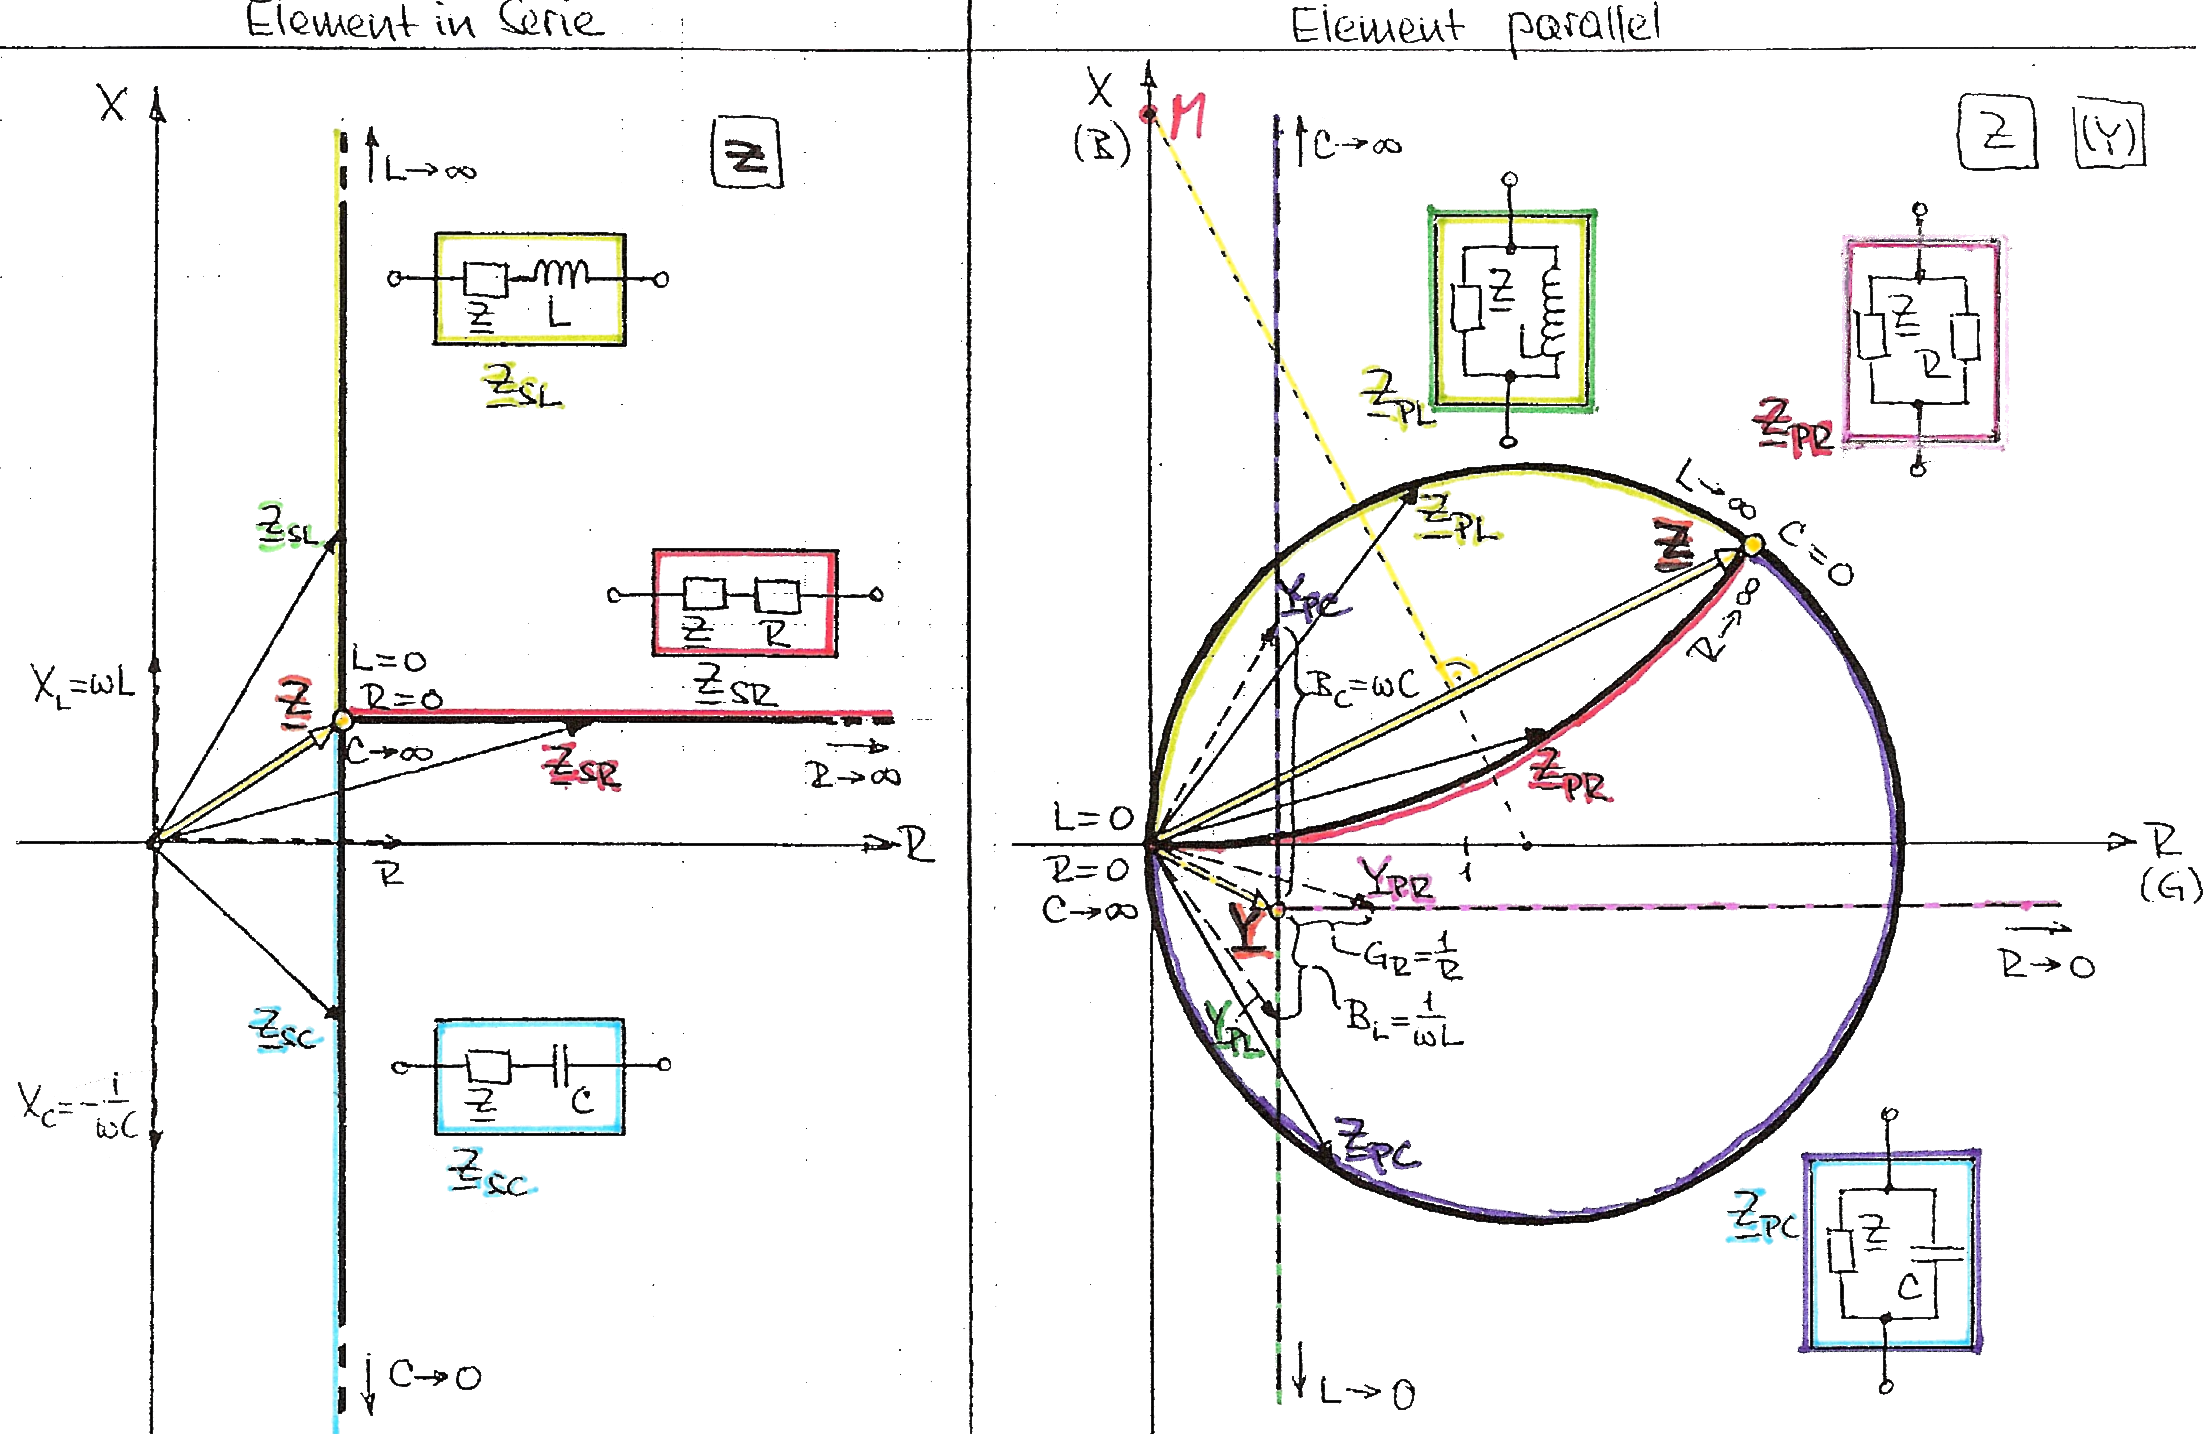
\includegraphics[width=18cm]{./images/impedanztrafo.png}